\documentclass[12pt,titlepage]{article}
\usepackage{graphicx}
\author{The TOME Team}
\title{\textbf{TOME Project Plan}}
\begin{document}
\maketitle
\tableofcontents
\listoffigures
\newpage
\section{Introduction}
\subsection{Purpose}
The purpose of this Project Plan is to document the \textbf{initial} plan for TOME.

It is emphasized that all sections of this document will be refined and expanded upon in later iterations of this Plan.

\subsection{Scope}
This document:
\begin{itemize}
	\item Lists the preliminary milestones for the project
	\item Gives preliminary dates for when milestones are to be completed
	\item States which milestones depend on other milestones
        \item Assigns milestones to specific people on the team
\end{itemize}
\section{Milestones}
\subsection{Definitions}
\subsubsection{Automated Test Suite}
This suite will be capable of creating a blank TOME database, starting a self-contained webserver, using the system like a normal user would, and checking the web and database output of the system.

The test suite milestone will have four checkpoints:
\begin{enumerate}
	\item Create an automated installation script. Currently, TOME installation must be done manually, and is complicated. This needs to change for the purposes of the test suite
	\item Integrate a self-contained Perl-based webserver for test purposes. The test suite should not depend on Apache being installed.
	\item Design a test framework. The capability to test should be independent from the individual tests.
	\item Write the tests. With the framework in place, the tests themselves can be written and deployed.
\end{enumerate}
\subsubsection{ISBN vs. ID}
All reservations will be made on an ISBN basis instead of for specific book IDs. Instead of reserving a specific, physical instance of a book, reservations will be made for ISBNs, and the database will ensure that the number of books reserved by ISBN does not exceed the number of physical books available. This will involve changes to the basic database structure as well as the code with which it interacts.
\subsubsection{Class-Based Verification}
In addition to the book verification TOME currently supports, class verification will be made available. This will allow TOMEkeepers to distinguish between classes which have no books and classes for which no books have been entered.
\subsubsection{Patron Page}
TOME will be reorganized to focus the entire work flow of selecting classes, reserving books, and making checkouts to be centered around patrons instead of books. This will make the job of the TOMEkeeper much easier.
\subsubsection{TOMEkeeper Page}
A page will be created with contact information for all current TOMEkeepers. The page will be generated dynamically from the database.
\subsubsection{UI Redesign}
The look and feel of TOME will be improved. The web interface will be refactored to be XHTML and CSS compliant, and any new workflows/pages required by other checkpoints will be created.
\subsection{Schedule}
\subsubsection{Automated Test Suite}
Due to the nature of this milestone, it will be developed throughout the entirety of the project, much in tandem with the rest of the project.  This is because specific requirements for the project have not yet been defined, and therefore cannot be tested.
\subsubsection{ISBN vs ID}
This Milestone began on September 12, and is scheduled to finish on September 19.
\subsubsection{Class-Based Verification}
Milestone to begin on September 19 and end on October 19.
\subsubsection{Patron Page}
Milestone to begin on October 19 and to end on November 14.
\subsubsection{TOME Keeper Page}
Milestone to begin on November 21 and to end on December 14.  This milestone is not required.
\subsubsection{UI Redesign}
This Milestone is much like the Automated Test Suite in that it needs to be developed in tandem with all other parts of the system, and is therefore not set with specific dates yet.
\subsection{Responsibilities}
\subsubsection{Automated Test Suite}
Clint Olson is responsible for this Milestone.
\subsubsection{ISBN vs ID}
Fjord (Curtis Hawthorne) is responsible for this Milestone.
\subsubsection{Class-Based Verification}
Fjord (Curtis Hawthorne) and fREW (Arthur Axel Schmidt) are responsible for this Milestone.
\subsubsection{Patron Page}
Fjord (Curtis Hawthorne) and fREW (Arthur Axel Schmidt) are responsible for this Milestone.
\subsubsection{TOME Keeper Page}
Fjord (Curtis Hawthorne) and fREW (Arthur Axel Schmidt) are responsible for this Milestone.
\subsubsection{UI Redesign}
Fargo (Craig Miller) is responsible for this Milestone.
\subsection{Dependencies}
\subsubsection{Automated Test Suite}
This milestone depends on all of the other milestones.  No other milestones depend on it.
\subsubsection{ISBN vs ID}
This Milestones is dependent on no other milestones.
\subsubsection{Class-Based Verification}
This milestone depends on the ISBN vs ID milestone.  The Patron Page directly depends on this Milestone.
\subsubsection{Patron Page}
This milestone directly depends on the Class Based Verification Milestone and the ISBN vs ID Milestone.  No Milestones directly depend on this milestone except for the ATS.
\subsubsection{TOME Keeper Page}
This Milestone depends on no other milestones but could be considered a part of the UI Redesign Milestone.
\subsubsection{UI Redesign}
The UI Redesign is an effort that can take place without other milestones being completed, but it will also be active in development on the Patron Page, the Class Based Verification, and the TOME Keeper Page.  As such it depends on others somewhat, but not entirely.
\section{GANTT Chart}
\begin{figure}[h]
	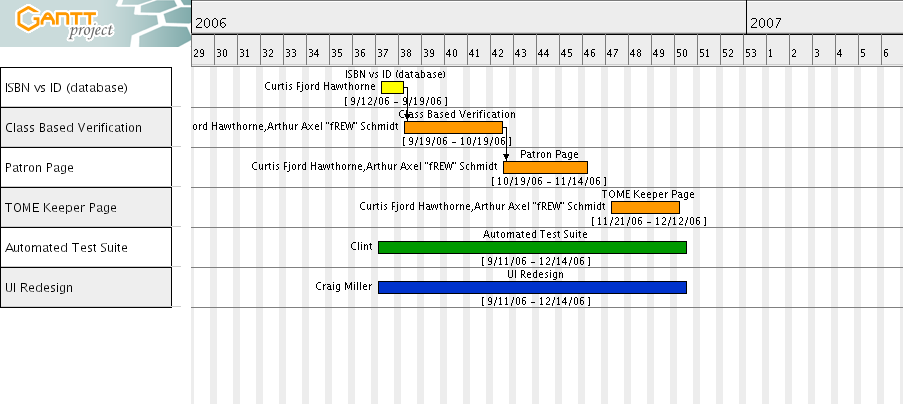
\includegraphics[width=\textwidth]{GanttChart}
	\caption{TOME Project GANTT Chart}
\end{figure}
\section{Overall Plan}
We are planning on doing this project in iterations.  What we will do is implement a feature and test it and document it, and then move on to another feature.  This way, we don't do 3 months worth of labor to find out that a low level error has been made and everything on top (everything) needs to be redesigned.
\end{document}
